\section{Introduction}

  Supersymmetry (SUSY) is an extension of the Standard Model which provides a solution to the hierarchy problem by explaining why the Higgs mass can be near the electroweak scale without
  excessive fine tuning. In models where $R$-parity\footnote{$R$ is defined as $R = (-1)^{3(B-L)+2s}$ in which $s$ is spin, $B$ is baryon number and $L$ is lepton number. The value
  of R is +1 for all Standard Model particles, while it is -1 for the supersymmetric particles. When $R$-parity is conserved, SUSY particles should be produced in pairs, and SUSY particles must decay into another SUSY particle.}
  is conserved~\cite{Wess:1974tw,Farrar:1978xj}, the lightest supersymmetric particle (LSP) is stable and could be a candidate for the dark matter observed by astrophysicists.
  Run I LHC data has provided strict limits on the production of generic colored superpartners using final states consisting of jets and missing energy. However, SUSY can still be natural (i.e. without 
  requiring fine-tuning of model parameters) if the
  superpartners of the Higgs boson, top quark, and gluon have masses near the electroweak scale~\cite{Barbieri:1987fn,deCarlos1993320,Dimopoulos1995573,Barbieri199676,Papucci:2011wy}. 
  New search strategies specifically targeted to these scenarios may provide stronger limits than generic searches.

  This note presents results of a search for scalar top partners produced in $pp$ collisions at a center-of-mass energy of $\sqrt{s}$ = 13 TeV. 
  As we focus on $R$-parity conserving models, the top squarks, denotes as \sTop, must always be produced in pairs $\sTop\PASQt$.
  These top squarks can have a variety of decay modes depending on the mass hierarchy of the SUSY particles. In this analysis, we consider the
  top squark decay mode $\sTop \to t\chiz_1$, where $t$ and $\chiz_1$ are the top quark and the lightest neutralino respectively. 
  This mode is represented by the Simplified Model Spectra (SMS)~\cite{Alwall:2008ag,Alwall:2008va,Alves:2011wf} labeled "T2tt" and is shown in Figure \ref{fig:T2tt}.

  \begin{figure}
    \centering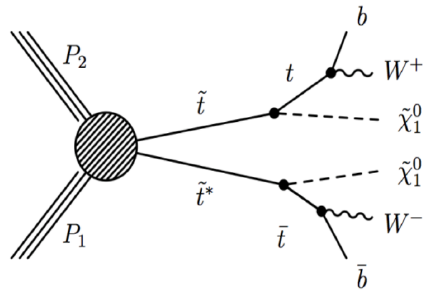
\includegraphics[width=10cm]{figures/T2tt.png}
    \caption{Diagram representing the simplified model "T2tt" of direct top squark production with decay via an on-shell top quark}
    \label{fig:T2tt}
  \end{figure}

  We use events with two opposite-sign isolated leptons, and two jets with at least one b-tagged jet to perform the search. The stransverse
  mass variable \mtll~\cite{Lester:1999tx} is used to separate the stop signal from the Standard Model background, which consists primarily of \ttbar decaying into dileptons.
  The stransverse mass is a generalization of the transverse mass \mt to a system of pair produced particles that decay semi-invisibly. 
  In the case of $W$ boson production, \mt is formed from the transverse momentum of a high \pt lepton (from the $W$ decay) and the missing transverse momentum (\met) in the event, 
  which is assumed to come from the corresponding neutrino. The definition of \mt in the limit where the masses of the daughter particles can be neglected is given by

  \begin{equation}
    \label{eq:mt}
    \mt = \sqrt{2 E_\ell \met \left[1 - \cos(\Delta\phi)\right]}
  \end{equation}

  The transverse mass has the property that if the lepton and the \met both come from the decay of a
  single particle with mass $m$, then $\mt \leq m$. In order to generalize to a system with two particles
  of the same mass, each decaying semi-invisibly, we have to decompose the measured \met into
  a sum of two missing transverse momentum vectors according to %as in Equation~\ref{eq:METsplit}:
 
  \begin{equation}
    \label{eq:METsplit}
    \mathbf{p}_T^{miss} = \mathbf{p}_{T1}^{miss} + \mathbf{p}_{T2}^{miss}.
  \end{equation}

  We may then pair each missing transverse momentum vector with the visible products of the
  decay in order to form \mt for each leg of the pair production. However, since the correct division of the \met into two components is not known, 
  a useful method is to minimize the maximum of the two transverse masses formed under all possible combinations satisfying Equation~\ref{eq:METsplit}. 
  That is, we explore the parameter space of all possible hypothetical neutrino momenta
  that satisfy Equation \ref{eq:METsplit} and for each point in this parameter space we calculate \mt for each half
  of the event and report the maximum of the two. We take the \mtll value for the event to be the
  minimum of the larger \mt value for each such point. This can be represented as %by the expression  for \mtll given in Equation~\ref{eq:mt2ll}:

  \begin{equation}
    \label{eq:mt2ll}
    M_{T2}^2(ll) = \min_{\mathbf{p}_{T1}^{miss} + \mathbf{p}_{T2}^{miss} = \mathbf{p}_T^{miss}} \left( \max \left[ \mt^2(\mathbf{p}_T^{\ell1},\mathbf{p}_{T1}^{miss}) , \mt^2(\mathbf{p}_T^{\ell2},\mathbf{p}_{T2}^{miss}) \right] \right)
  \end{equation}

  It can be shown~\cite{Lester:1999tx} that this definition of \mtll has the same convenient property as the transverse mass: 
  it must be less than the mass of the pair-produced semi-invisibly decaying particle.
  In the case of stop ($\sTop \to t\chiz_1$) searches in the dilepton channel, the primary challenge comes from separating SM \ttbar 
  production from the signal, since the composition of the final states is identical except
  for invisible particles. In dileptonic \ttbar events the final state is

  \begin{equation*}
    pp \to t + \bar{t} + X \to bW^+ + \bar{b}W^- + X \to b\ell\bar{\nu}_\ell + \bar{b}\bar{\ell}\nu_\ell + X.  
  \end{equation*}

  Assuming that the contribution of the other products $X$ to the \met is not large, the assumptions
  made in the definition of \mtll hold for the lepton-\met system and its value has an upper
  bound at the $W$ mass. On the other hand, stop pair production events with a dileptonic final
  state will have at least four invisible particles so long as lepton number and $R$-parity are both
  conserved. The stop decays can proceed differently depending on the model considered but a
  typical example for the models used here is

  \begin{equation*}
    pp \to \tilde{t} + \bar{\tilde{t}} + X \to \bar{\chiz_1}t + \chiz_1\bar{t} + X \to \bar{\chiz_1}bW^+ + \chiz_1\bar{b}W^- + X \to \bar{\chiz_1}b\ell\bar{\nu}_\ell + \chiz_1\bar{b}\bar{\ell}\nu_\ell + X.  
  \end{equation*}

  Now there are
  two invisible particles on each side of the decay, and so the partition of the
  \met into two components no longer has an upper bound at the W mass.

  Similarly, one is also able to construct two other variants on the \mtll variable, which take into account the $b$-jets and are expected to have an upper bound at the top mass:

  \begin{align}
    \label{eq:mt2bb}
    M_{T2}^2(bb)   &= \min_{\mathbf{p}_{T1}^{miss} + \mathbf{p}_{T2}^{miss} = \mathbf{p}_T^{miss}} \left( \max_{b \in b_1,b_2} \left[ \mt^2(\mathbf{p}_T^{b},\mathbf{p}_{T1}^{miss}) \right] \right) \\
    M_{T2}^2(lblb) &= \min_{\mathbf{p}_{T1}^{miss} + \mathbf{p}_{T2}^{miss} = \mathbf{p}_T^{miss}} \left( \max_{b \in b_1,b_2, \ell \in \ell_1, \ell_2} \left[ \mt^2(\mathbf{p}_T^{b} + \mathbf{p}_T^{\ell}, \mathbf{p}_{T1}^{miss}) \right] \right)
  \end{align}
  There are two choices how to pair the two leptons  and the two b-jets in the case of \mtlblb. This ambiguity is resolved by minimizing the maximum invariant mass of the two lepton-jet pairs.

  The analysis strategy described in the note uses this property of \mtll, \mtbb and \mtlblb in order to construct
  signal regions, with $\mtll > M_W$, that should have a small
  contamination from dileptonic top decays stemming from the Standard Model.
